%!TEX root = ../../thesis.tex
\section{Idea}

\begin{figure}[h]
  \centerline{
    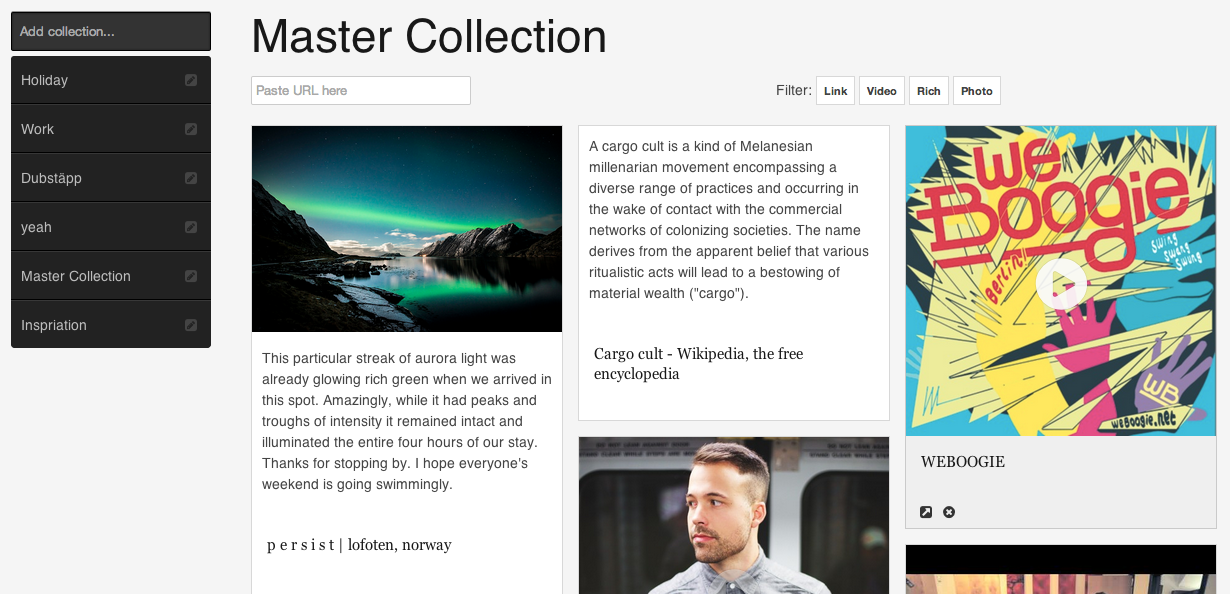
\includegraphics[width=\linewidth]{images/collection-screen.png}
  }
  \caption[collection.do main screen]{collection.do main screen}
  \label{fig:collection-screen}
\end{figure}

\textbf{collection.do}\footnote{The code for this example can be found at \url{https://github.com/janmonschke/Angular-Book/tree/master/collection-do}. The page is hosted at \url{http://collection.janmon.libra.uberspace.de}.} is a web service that allows to collect arbitrary multimedia content form various web sources and to organize the collected bits of content into collections. Users can add content using its URL and the backend then fetches rich previews of the content. Collection.do in its current form can be seen as a combination of delicious\footnote{\url{https://delicious.com}, last-checked on 22/04/2014}, a social bookmarking service, and Pinterest\footnote{\url{https://pinterest.com}, last-checked on 22/04/2014}, a visual content aggregation tool. It is however in this version not intended for sharing content with others or to discover web resources. It is much more a tool to create private collections e.g. for brain storming or to organize events. Future versions of collection.do will have a sharing feature and an aggregation feature to allow users to collaboratively work on collections.

In \reffigure{fig:collection-screen} the layout of collection.do is shown. There is a list of collections on the left side. By clicking one of these entries, the user will be presented with the content of that collection. New collections can be added by using the form field on the top. The name of a collection can be changed by clicking the edit-button on the right. A collection's content is presented as individual cards that show a preview of the linked content (e.g. an image or a text abstract). The linked multimedia content can easily be embedded by clicking the play button. On the bottom of each card, the user is able to delete the card or to jump to the original content. The top of the content pane shows the collection's title and allows the user to add content to the page. Furthermore, the buttons on the right allow to filter the collection's content by type.